\subsection{Cartesian squares}

Let B, B′, X, X′ be topological spaces and let \(f: B' \to B\) , \(f': X' \to X\) , \(p: X \to B\) , \(p': X' \to B'\) be continuous maps. One can represent such a quadruple \((f, f', p, p')\) by a diagram

\begin{enumerate}
\def\labelenumi{(\arabic{enumi})}
\tightlist
\item
\end{enumerate}

\pandocbounded{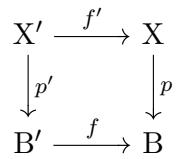
\includegraphics[keepaspectratio]{images/part001_dd3067cf.jpg}}

(E, II, p. 14). We shall then say, “Consider the square diagram (1),” or simply “the square (1),” instead of saying, “Consider the quadruple \(f,f^{\prime},p,p^{\prime}\) of continuous maps.” The square (1) is said to be commutative if the equality

\[
f \circ p ^ {\prime} = p \circ f ^ {\prime}
\]

is satisfied. In this case, one often endows B′, X, and X′ with the structures of B-spaces defined by the maps f, p, and \(f \circ p' = p \circ f'\) respectively; the maps \(p'\) and \(f'\) are then B-morphisms.

DEFINITION 4. --- We say that the square (1) is a Cartesian square of topological spaces (or, simply, that it is Cartesian) if it is commutative and if, for every topological space Y and every pair of continuous maps u: Y → B', v: Y → X such that f ∘ u = p ∘ v, there exists a unique continuous map w: Y → X' such that p' ∘ w = u and f' ∘ w = v.

For the square (1) to be Cartesian, it is necessary and sufficient that the square

(1')

\pandocbounded{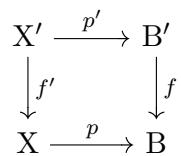
\includegraphics[keepaspectratio]{images/part001_f0fdde30.jpg}}

is Cartesian.

PROPOSITION 1. --- For the square (1) to be Cartesian, it is necessary and sufficient that it be commutative and that, for every B-space Y and every pair of B-morphisms \(u\colon Y \to B'\) , \(v\colon Y \to X\) there exists a unique B-morphism \(w\colon Y \to X'\) such that \(p' \circ w = u\) and \(f' \circ w = v\) .

Suppose that the square (1) is Cartesian. Let Y be a B-space and let \(u: Y \to B'\) and \(v: Y \to X\) be B-morphisms. The maps \(f \circ u\) and \(p \circ v\) are both equal to the projection of the B-space Y; the unique continuous map w such that \(p' \circ w = u\) and \(f' \circ w = v\) is then a B-morphism. This proves the necessity of the condition.

Conversely, suppose this condition is satisfied. Let Y be a topological space and let \(u \colon \mathrm{Y} \to \mathrm{B}'\) and \(v \colon \mathrm{Y} \to \mathrm{X}\) be continuous maps such that \(f \circ u = p \circ v\) . When Y is endowed with the B-space structure defined by \(f \circ u\) , \(u\) and \(v\) are B-morphisms. Every continuous map \(w \colon \mathrm{Y} \to \mathrm{X}'\) such that \(p' \circ w = u\) and \(f' \circ w = v\) is a B-morphism, so there exists exactly one such map.

PROPOSITION 2. --- Let B, B' and X be topological spaces and p: X → B, f: B' → B continuous maps.

\begin{enumerate}
\def\labelenumi{\alph{enumi})}
\tightlist
\item
  The square
\end{enumerate}

\[
\begin{array}{c} \mathrm{B} ^ {\prime} \times_ {\mathrm{B}} \mathrm{X} \xrightarrow {\mathrm{pr} _ {2}} \mathrm{X} \\ \Biggl \downarrow \mathrm{pr} _ {1} \\ \mathrm{B} ^ {\prime} \xrightarrow {f} \mathrm{B} \end{array}\tag{2}
\]

is a Cartesian square.

\begin{enumerate}
\def\labelenumi{\alph{enumi})}
\setcounter{enumi}{1}
\tightlist
\item
  For every commutative square
\end{enumerate}

\[
\begin{array}{c} \mathrm {X^ {\prime}} \xrightarrow {f ^ {\prime}} \mathrm{X} \\ \Big \downarrow_ {p ^ {\prime}} \\ \mathrm {B^ {\prime}} \xrightarrow {f} \mathrm{B} \end{array}\tag{3}
\]

there exists a unique continuous map \(h: X' \to B' \times_{B} X\) such that \(pr_{1} \circ h = p'\) and \(pr_{2} \circ h = f'\) .

\begin{enumerate}
\def\labelenumi{\alph{enumi})}
\setcounter{enumi}{2}
\tightlist
\item
  The commutative square (3) is Cartesian if and only if h is a homeomorphism.
\end{enumerate}

Assertion \(a\) ) follows from Proposition 1 and the universal property of the product of two B-spaces in the category of B-spaces (I, p. 3). Assertion \(b\) ) follows from it.

If the square (3) is Cartesian, there exists a unique continuous map \(h'\colon B'\times_{B}X\to X'\) such that \(f'\circ h' = pr_{2}\) and \(p'\circ h' = pr_{1}\) . We have \(f'\circ h'\circ h = f'\) and \(p'\circ h'\circ h = p'\) , whence \(h'\circ h = Id_{X'}\) since the square (3) is Cartesian. We have \(pr_{1}\circ h\circ h' = pr_{1}\) and \(pr_{2}\circ h\circ h' = pr_{2}\) , whence \(h\circ h' = Id_{B'\times_{B}X}\) since the square (2) is Cartesian. This proves that h is a homeomorphism.

Conversely, suppose that h is a homeomorphism; since square (2) is Cartesian, square (3) is also Cartesian.

The map \(h \colon \mathrm{X}' \to \mathrm{B}' \times_{\mathrm{B}} \mathrm{X}\) whose existence and uniqueness is asserted by part \(b)\) of the preceding proposition will be called canonical: it is the map denoted \((p', f')\) in I, p. 3.

PROPOSITION 3. --- Let

\[
\begin{array}{c} \mathrm {X^ {\prime}} \xrightarrow {f ^ {\prime}} \mathrm{X} \\ \Big \downarrow_ {p ^ {\prime}} \\ \mathrm {B^ {\prime}} \xrightarrow {f} \mathrm{B} \end{array}
\]

a Cartesian square. For any continuous section s of \(p'\) , the map \(f'\circ s\) is a continuous lift of f to X. The map \(s\mapsto f'\circ s\) is a bijection from \(\mathcal{C}_{\mathrm{B}'}(\mathrm{B}';\mathrm{X}')\) onto \(\mathcal{C}_{\mathrm{B}}(\mathrm{B}';\mathrm{X})\) .

If \(s \colon B' \to X'\) is a continuous section of \(p'\) , we have \(p \circ f' \circ s = f \circ p' \circ s = f\) , which proves that \(f' \circ s\) is a continuous lifting of \(f\) to X, i.e., a B-morphism from \(B'\) into X. Conversely, let \(g \colon B' \to X\) be a B-morphism. We have \(f \circ \mathrm{Id}_{\mathrm{B}'} = p \circ g\) ; there therefore exists, by definition of a Cartesian square, a unique continuous map \(s \colon B' \to X'\) such that \(p' \circ s = \mathrm{Id}_{\mathrm{B}'}\) and \(f' \circ s = g\) , whence the proposition.

